% CVPR 2023 Paper Template
% based on the CVPR template provided by Ming-Ming Cheng (https://github.com/MCG-NKU/CVPR_Template)
% modified and extended by Stefan Roth (stefan.roth@NOSPAMtu-darmstadt.de)

\documentclass[10pt,twocolumn,letterpaper]{article}

%%%%%%%%% PAPER TYPE  - PLEASE UPDATE FOR FINAL VERSION
\usepackage{cvpr}      % To produce the REVIEW version


% Include other packages here, before hyperref.
\usepackage{graphicx}
\usepackage{amsmath}
\usepackage{amssymb}
\usepackage{booktabs}


% It is strongly recommended to use hyperref, especially for the review version.
% hyperref with option pagebackref eases the reviewers' job.
% Please disable hyperref *only* if you encounter grave issues, e.g. with the
% file validation for the camera-ready version.
%
% If you comment hyperref and then uncomment it, you should delete
% ReviewTempalte.aux before re-running LaTeX.
% (Or just hit 'q' on the first LaTeX run, let it finish, and you
%  should be clear).
\usepackage[pagebackref,breaklinks,colorlinks]{hyperref}


% Support for easy cross-referencing
\usepackage[capitalize]{cleveref}
\crefname{section}{Sec.}{Secs.}
\Crefname{section}{Section}{Sections}
\Crefname{table}{Table}{Tables}
\crefname{table}{Tab.}{Tabs.}


%%%%%%%%% PAPER ID  - PLEASE UPDATE
\def\cvprPaperID{*****} % *** Enter the CVPR Paper ID here
\def\confName{CVPR}
\def\confYear{2023}


\begin{document}

%%%%%%%%% TITLE - PLEASE UPDATE
\title{Team \#16: From Strings to Sequences --- Classifying and Generating Music from Acoustic Guitar Notes}

\author{
Camilo Martínez\\
7057573\\
\and
Dhimitrios Duka\\
7059153\\
\and
Honglu Ma\\
7055053\\
}
\maketitle

%%%%%%%%% BODY TEXT
\section{Task and Motivation}
Automatic cord recognition (ACR) has been getting more attention in the last years. ACR aims to extract chord information which can later on be used to analye the given music piece. ACR was first introduced in 1999 by \cite{} and since then, many different approaches have been proposed. At first most of them \cite{} approached this task from an audio signal processing. With the rise of deep learning, many researches started to use deep learning models to solve this task.  


The task consists of recognizing the chord being played in a music piece. This task is important for music analysis, music transcription, and music information retrieval. The task is challenging due to the high variability of the guitar playing, the presence of noise, and the high number of classes. The task can be divided into two subtasks: fretboard detection and chord recognition. Fretboard detection consists of detecting the fretboard in an image, while chord recognition consists of recognizing the chord being played.

Task statement and definitions

Motivation: Why do we need to explore this task?

Related work: How do existing papers solve this task or similar tasks (should include relevant citations)?

Challenge: What are the major challenges that have not been solved in this task?

\cite{Kristian_Zaman_Tenoyo_Jodhinata_2024}
\cite{du2023conditional}

\section{Goals}

What challenges do you aim to address in this task?

What do you want to have completed by the mid-term? E.g., code for the task, data collection, results for baselines, etc.


\begin{figure*}[h]\label{fig:diagram}
    \centering
    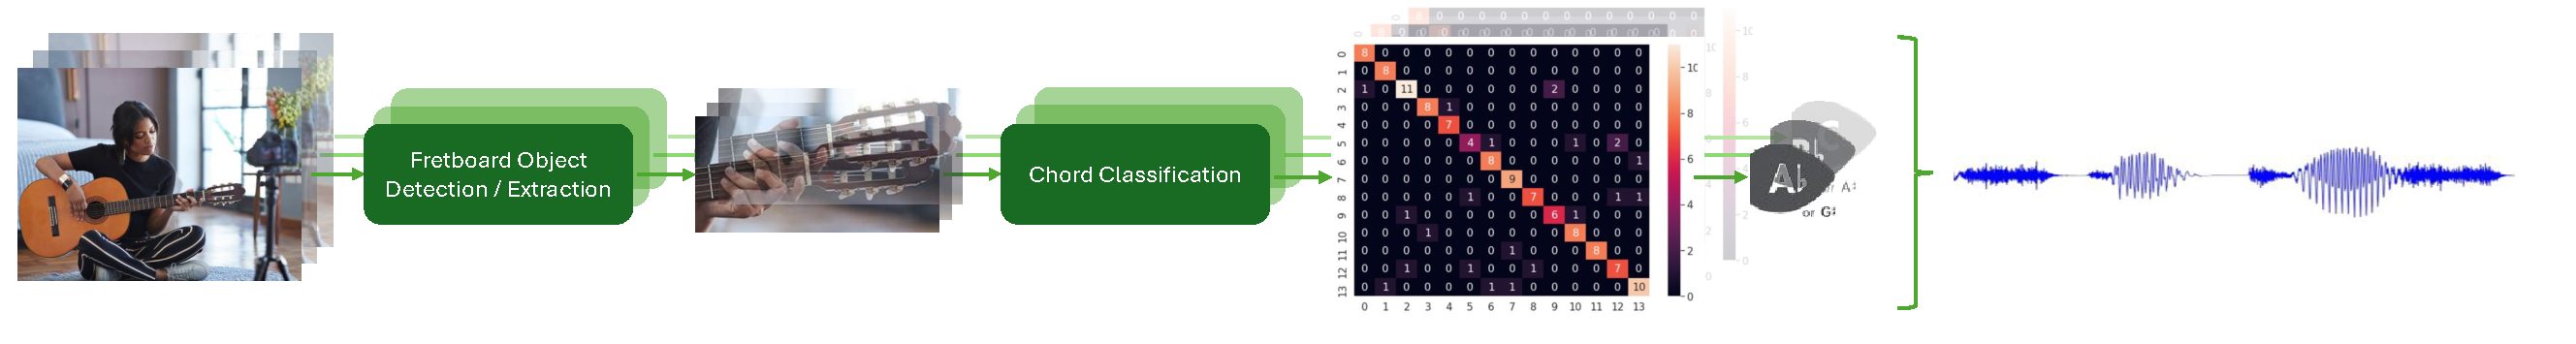
\includegraphics[width=\textwidth]{images/task-diagram.pdf}
    \caption{Example figure.}
    \label{fig:figure1}
\end{figure*}


\section{Methods}

What models/frameworks do you use to solve the challenges?

Why can the proposed method / analysis solve your problem?

What are the main differences between your method and existing methods (if applicable)?

What is the required computational budget for the training/analysis? (E.g. are you planning on using pretrained backbones?)

\section{Datasets}

What datasets are you going to use/collect and why?


\subsection{Fretboard Detection}
This one has both: \cite{guitar-chords-daewp_dataset}. 
Only fretboard: \cite{guitar-ppfil_dataset}, \cite{done-npcll_dataset}.

\subsection{Chord Recognition}
For chord recognition: \cite{guitar-chord-tvon8_dataset}, \cite{guitar-chord-bounding-box_dataset}, \cite{guitar-chord-handshape_dataset}.

\section{Evaluation}

How is your method going to be evaluated?

What metrics are suitable?

Do you need to define your own metric for evaluation?

\clearpage 

%%%%%%%%% REFERENCES
{\small
\bibliographystyle{ieee_fullname}
\bibliography{references}
}

\end{document}
